\section{Component Diagram}

A partire dai casi d’uso, è stata progettata l’architettura del sistema seguendo un’organizzazione a più livelli, al fine di separare chiaramente interfaccia utente, logica applicativa e persistenza dei dati. Questa suddivisione consente di ottenere un sistema modulare ed estendibile.

\begin{figure}[H]
    \centering
    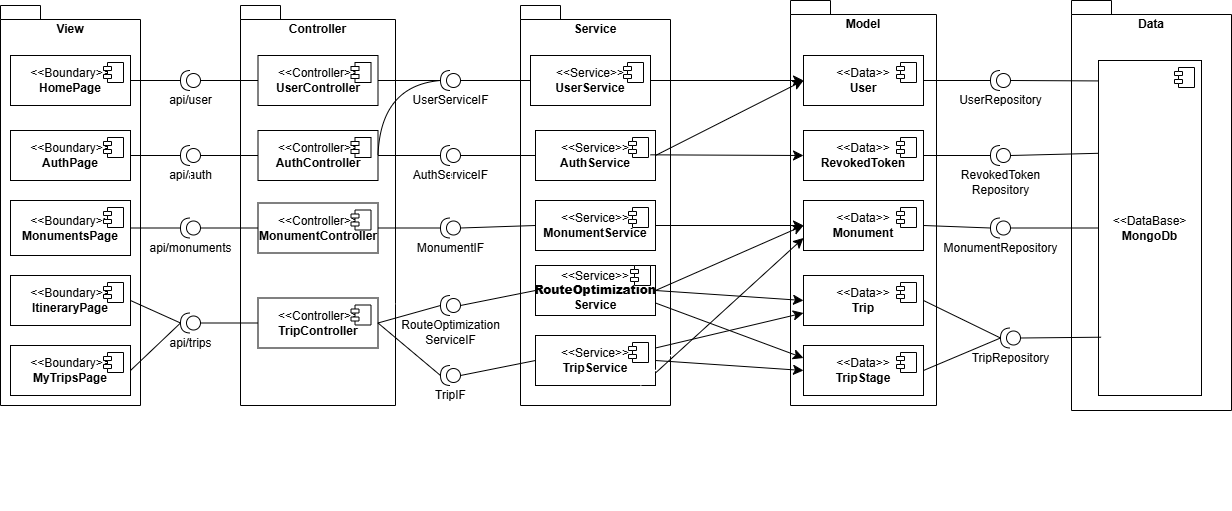
\includegraphics[width=\linewidth]{Iterazione1/Diagrammi/ComponentDiagram.png}
    \caption{Diagramma dei componenti}
    \label{fig:ComponentDiagram}
\end{figure}

Il diagramma è strutturato in cinque livelli principali: \textit{View}, \textit{Controller}, \textit{Service}, \textit{Model} e \textit{Data}. 

\begin{itemize}
    \item \textbf{\textit{View}}: rappresenta i componenti \textit{boundary} del front-end, ovvero le pagine con cui l’utente interagisce direttamente: \textit{HomePage}, \textit{AuthPage}, \textit{MonumentsPage}, \textit{ItineraryPage} e \textit{MyTripsPage}. Questi componenti comunicano con il backend attraverso le API esposte dai controller.
    
    \item \textbf{\textit{Controller}}: contiene i componenti che ricevono le richieste HTTP e le indirizzano verso la logica applicativa appropriata. Il sistema espone endpoint distinti per la gestione degli utenti, dell’autenticazione, dei monumenti e dei viaggi: \textit{UserController}, \textit{AuthController}, \textit{MonumentController} e \textit{TripController}.
    
    \item \textbf{\textit{Service}}: include la logica di business del sistema. I controller delegano a questi componenti l’esecuzione delle operazioni principali attraverso interfacce dedicate, quali \textit{UserServiceIF}, \textit{AuthServiceIF}, \textit{MonumentIF}, \textit{RouteOptimizationServiceIF} e \textit{TripIF}. Le rispettive implementazioni, ovvero \textit{UserService}, \textit{AuthService}, \textit{MonumentService}, \textit{RouteOptimizationService} e \textit{TripService}, si occupano di gestire i dati e le funzionalità del sistema. In particolare, la gestione dei viaggi distingue tra gestione del viaggio e ottimizzazione del percorso.
    
    \item \textbf{\textit{Model}}: definisce le entità del dominio, che rappresentano gli oggetti principali gestiti dall’applicazione: \textit{User}, \textit{RevokedToken}, \textit{Monument}, \textit{Trip} e \textit{TripStage}. Queste classi costituiscono il modello dei dati utilizzato dai service e dal database.
    
    \item \textbf{\textit{Data}}: comprende i componenti responsabili dell’accesso al database, ovvero i repository \textit{UserRepository}, \textit{RevokedTokenRepository}, \textit{MonumentRepository} e \textit{TripRepository}, tutti collegati al database \textit{MongoDb}. Questo livello gestisce le operazioni di lettura e scrittura, mantenendo separata la logica di accesso ai dati dalla logica applicativa.
\end{itemize}

Nel complesso, il diagramma presenta una struttura coerente con il principio di separazione delle responsabilità: le componenti di \textit{View} interagiscono con i \textit{Controller}, i \textit{Controller} delegano ai \textit{Service} la logica di business, i \textit{Service} utilizzano le entità del \textit{Model} e accedono ai dati tramite il livello \textit{Data}. Questa organizzazione rende l’architettura chiara e robusta.